

\documentclass[oneside,20pt]{article}          % please do not change
\usepackage[b5paper]{geometry}	    % your paper can be easily printed on a4 or letter paper with enlargenment      
                                    % comment if you have problem with print     
\usepackage{amsfonts,amsmath,latexsym,amssymb}
\usepackage{graphicx}
%%% remove comment delimiter ('%') and specify parameters if required
%\usepackage[dvips]{graphics}

\begin{document}

%%% remove comment delimiter ('%') and select language if required
%\selectlanguage{spanish} 

\noindent 
\begin{center}
  \texttt{LABORATOR 4-- Hacking cu Python.}        
\end{center}

\section{WEB Hacking}
\noindent                 
\\\\\
Majoritatea serviciilor pe care le utilizați funcționează prin Internet. În
în special, paginile web transmise prin protocolul HTTP pot fi la inima unui serviciu de internet. O pagină de pornire care este utilizată pentru un computer
iar un smartphone este un fel de serviciu Web. Majoritatea companiilor, practic blocheaza toate porturile de serviciu din cauza securității, dar portul 80 rămâne deschis pentru Servicii web. Google, care este un portal tipic pe care oamenii se conectează la zi de zi, folosește și portul 80. Serviciile web recunosc asta
utilizați portul 80, dacă nu specificați un alt port în spatele URL-ului. Prin portul 80, un server web transmite o varietate
de date pe computer, inclusiv text, imagini, fișiere, videoclipuri. Prin portul 80, un utilizator poate transmite, de asemenea, o varietate de date de la text la un mare fișier pe un server web. Diagrama conceptuala a accesului pe Net o prezentam mai jos:
\begin{center}
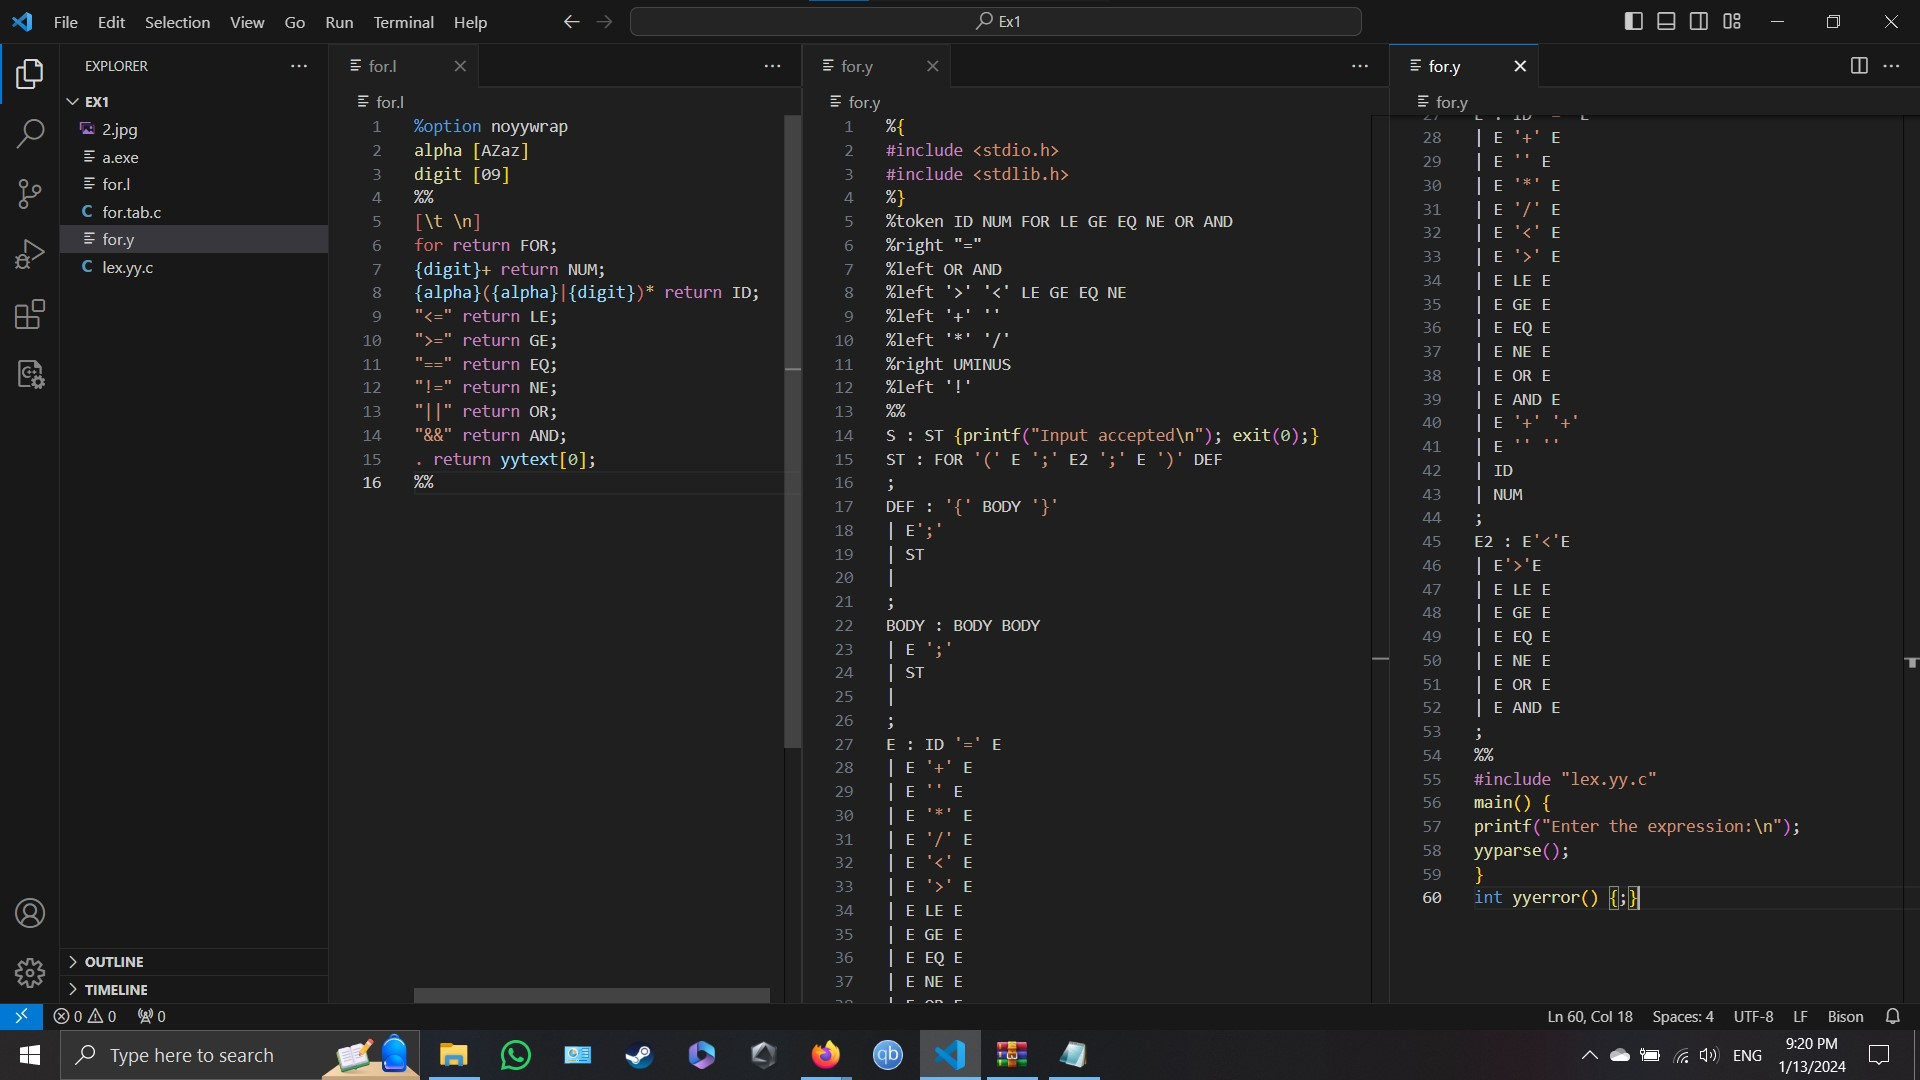
\includegraphics[height = 5 cm]{1.png}
\end{center}

Portul 80 poate fi utilizat într-o varietate de moduri. Cu toate acestea, un firewall o face
in asa fel incat sa nu efectuați o verificare de securitate pe portul 80. Pentru a rezolva aceasta 
vulnerabilitate, poate fi implementat un Web Firewall. Cu toate acestea, este
imposibil de protejat de toate atacurile, care evoluează în fiecare zi. In acest moment, hackerii exploatează vulnerabilitățile din serviciile Web
și încearcă să conducă atacuri fatale.
OWASP (The Open Web Application Security Project) analizeaza vulnerabilități de securitate pe web anual. OWASP publică a
Top 10 vulnerabilitati, iar detaliile sunt următoarele:
•\textbf{A1 Injecție}\\
Un hacker efectuează un atac prin injecție folosind date nesigure
la transferul de instrucțiuni către baze de date, sisteme de operare,
LDAP. Hackerii execută o comandă de sistem printr-un
atac de injecție pentru a obține acces la date neautorizate.\\
•\textbf{ A2 Broken Authentication and Session Management}\\
Programatorii dezvoltă autentificarea și gestionarea sesiunilor
funcțiile în sine, iar programatorii calificați pot crea un
functioneaza in siguranta. Cu toate acestea, se dezvoltă programatori fără experiență
funcții care sunt vulnerabile la hacking. Hackerii fură
parolele care utilizează aceste vulnerabilități sau chiar ocolesc
autentificarea cu totul.\\
• \textbf{A3 Cross-Site Scripting (XSS)}\\
O vulnerabilitate XSS apare atunci când o aplicație trimite date către
un browser web fără validare adecvată. Importante
informații de pe PC care fuseseră introduse de victima care a
executat scriptul XSS sunt apoi transmis hackerului.\\
• \textbf{A4 Insecure Direct Object References}\\
Într-un mediu în care măsurile de securitate adecvate au
luat, un utilizator nu poate accesa obiecte interne, astfel de fișiere,
directoare și chei de bază de date prin intermediul unui URL. Doar prin auxiliar
înseamnă că este posibil să accesezi obiecte interne. Dacă un intern
obiectul este expus direct utilizatorului, este posibil să fie accesat
date neautorizate prin operarea metodei de acces.\\
• \textbf{A5 Security Misconfiguration}\\
Aplicațiile, cadrele, serverele de aplicații, serverele web,
serverele de baze de date și platformele au implementat o varietate de
tehnologii de securitate. Un administrator poate schimba securitatea
nivel prin modificarea fișierului de mediu. Tehnologia de securitate
care a fost instalata poate fi expusa unui nou atac peste
timp. Pentru a menține siguranța sistemului, 
administratorul trebuie să verifice în permanenţă mediul şi
trebuie să se asigure că software-ul este actualizat.\\
• \textbf{A6 Sensitive Data Exposure}\\
Aplicațiile web utilizează diverse forme de date importante,
inclusiv informații private și informații de autentificare. A
programatorul trebuie să ia măsuri de protecție, cum ar fi criptarea
date, atunci când stocați sau transferați date sensibile.
• \textbf{A7 Missing Function Level Access Control}\\
Din motive de securitate, trebuie să verificați permisiunile pe Web
ale aplicațiilor pe partea de server. Din când în când, dezvoltatori
fac greșeala să verifice permisiunile cu un script pe 
partea clientului. Un web scroller este un program care găsește adresa URL a unui
server web și analizează apelul HTML. Permisiunile care
sunt procesate de script pot fi verificate ca au fost
neutralizate de un web scroller.\\
• \textbf{A8 Cross-Site Request Forgery (CSRF)}\\
Hackerul creează un script care conține funcții pentru a ataca a
site-ul specific și îl publică pe Internet. Când o victimă
face clic pe pagina web în care este încorporat scriptul CSRF,
scriptul va ataca alte site-uri fără știrea utilizatorului.\\
• \textbf{A9 Using Components with Known Vulnerabilities}\\
Serverul are componente care rulează folosind privilegii root. Dacă există
hackerul poate obține acces la astfel de componente, poate duce la
consecințe serioase. Prin urmare, este foarte important să luați
măsuri adecvate împotriva vulnerabilităților de securitate care
au fost raportate pentru componente.\\
• \textbf{A10 Unvalidated Redirects and Forwards}\\
Unele scripturi sunt capabile să mute forțat paginile care sunt ale utilizatorului.
Majoritatea atacurilor de hacking pot fi blocate folosind un firewall, IDS, IPS sau o
firewall aplicație web. Cu toate acestea, hacking-ul de pe web este greu de blocat
deoarece utilizează un serviciu web normal și un port deschis 80.
În mod realist, hacking-ul web este cel mai simplu mod prin care să faci
implementari la o tehnică de hacking. Este mai puternic decât orice alta
tehnica de hacking. O injecție SQL, spargerea de parole și  atacul Shell se află în fruntea listei OWASP Top 10. Acum, să ne uităm
la aceste tehnici de hacking folosind Python.\\
Pentru a efectua un test de hacking al unei rețele, este necesar să aveți
diverse PC-uri. În special pentru testul de hacking web, este necesar să
construiti un server Web și o bază de date. Este oarecum scump să
investiți în astfel de echipamente doar pentru un studiu de hacking. Prin urmare,
tehnologia de virtualizare și software-ul open source pot fi folosite pentru
rezolvarea acestei probleme. Mai întâi, să examinăm tehnologia de virtualizare
pe care o vom folosi. Oracle oferă un utilitar software numit Virtual Box
care este gratuit pentru utilizare pe computer. Virtual Box poate fi folosit pentru a instala
diverse sisteme de operare pe o mașină virtuală, care pot fi folosite pentru
ca funcționează ca un computer separat.
\begin{center}
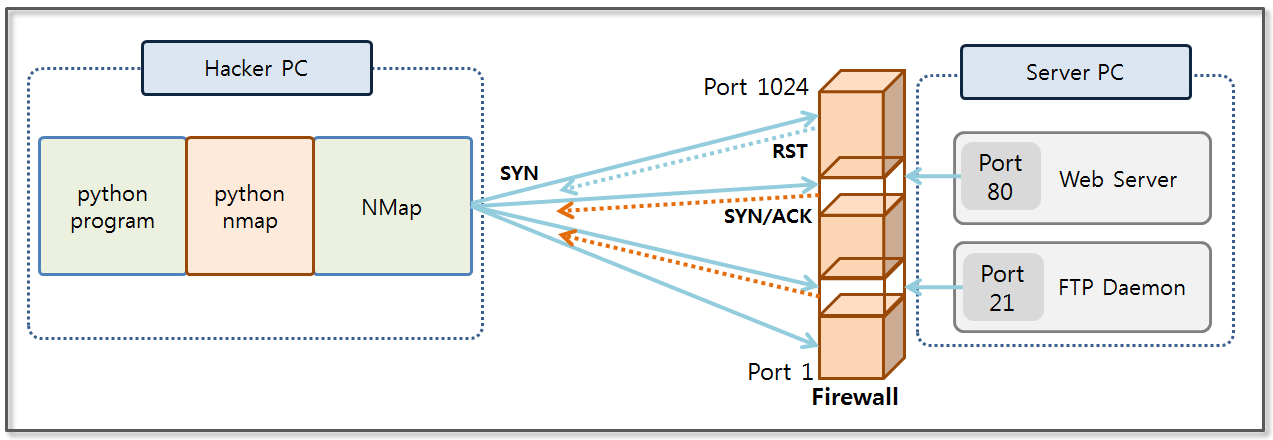
\includegraphics[height = 3 cm]{2.png}
\end{center}
Instalați Apache și Mysql pentru a utiliza serverul Web și DB. Tu
le pot folosi gratuit deoarece sunt open source. Instalați un PHP bazat
Site WordPress open source pentru hacking. Acest software acceptă funcțiile de blogging.
\begin{center}
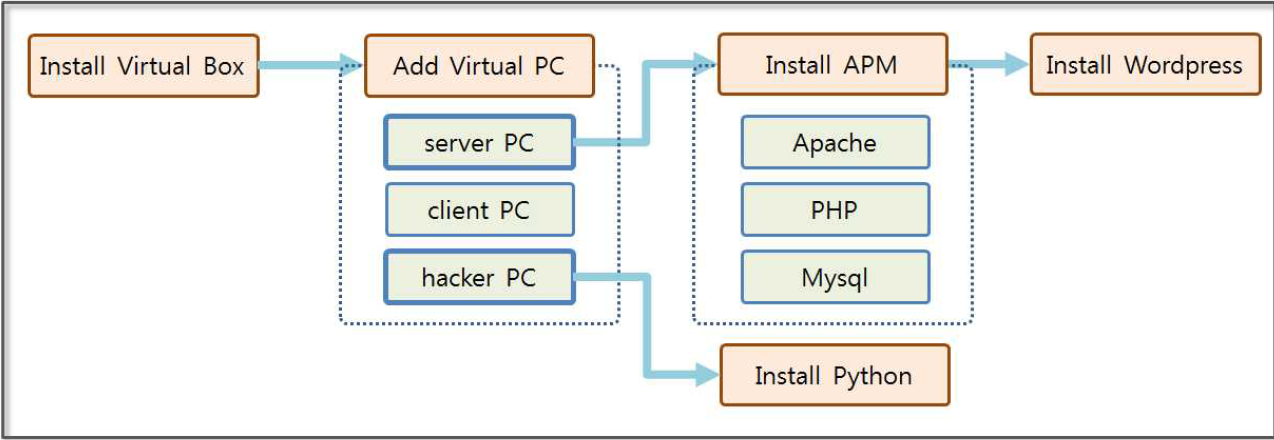
\includegraphics[height = 3 cm]{3.png}
\end{center}
\textbf{Injecție SQL (SQL Injection)}\\
Atacurile SQL Injection pot fi efectuate prin inserarea unui SQL anormal
cod într-o aplicație vulnerabilă pentru ca programul să ruleze anormal.
Această formă de atac este efectuată în principal prin introducerea codului de hacking
într-o variabilă care primește și procesează intrarea utilizatorului.

Cod general de autentificare a utilizatorului
\begin{center}
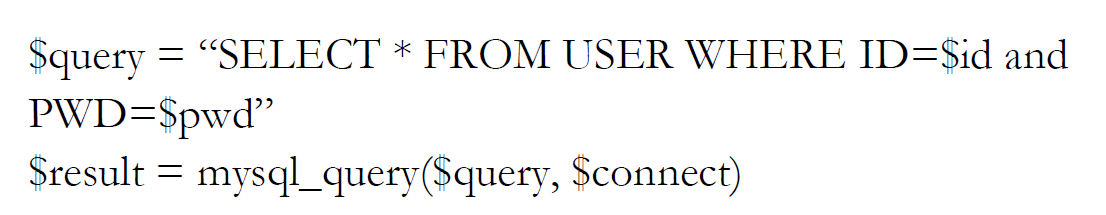
\includegraphics[height = 1 cm]{4.png}
\end{center}
De obicei, utilizatorii se conectează folosind numele de utilizator și parola. Dacă utilizatorul
folosește numele de utilizator și parola corecte, serverul Web cu succes finalizează procesul de autentificare. Să introducem SQL anormal.\\
Codați în câmpul ”id” pentru a efectua o injecție SQL.
 Cod de injectare SQL\\
$$1 OR 1=1 --$$

Dacă codul de mai sus este introdus în câmpul ”id”, SQL-ul normal
declarația se modifică după cum urmează.\\
\textbf{Declarație SQL modificată}\\
\begin{center}
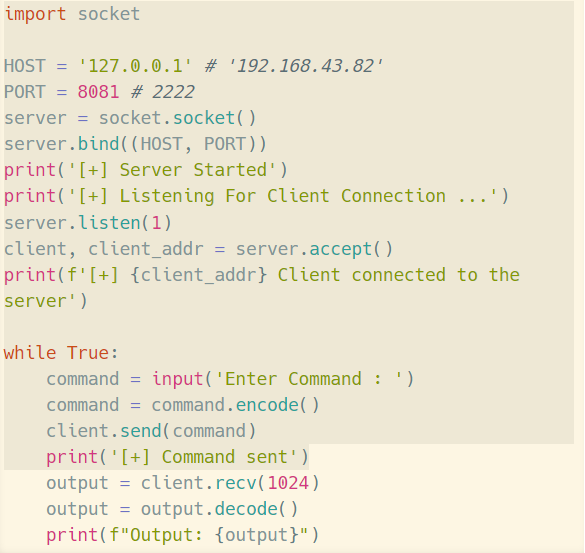
\includegraphics[height = 1 cm]{5.png}
\end{center}
Dacă introduceți ”ID = 1 SAU 1 = 1” într-o declarație condiționată,
baza de date va tipări toate informațiile legate de utilizatori. Parola este
comentata cu ”--”. Prin urmare, instrucțiunea SQL care se ocupă
autentificarea utilizatorului este dezactivată. Pentru a finaliza un SQL de succes
Injectare, este necesar să se introducă diverse valori, iar acestea repetitive
sarcinile pot fi automatizate prin scrierea unui program. Python oferă o
varietate de module care pot automatiza aceste sarcini, cu sqlmap ca si caz reprezentativ.
Acum, să instalăm sqlmap. Descărcați fișierul zip conectându-vă la
http://sqlmap.org. Dezarhivați fișierul în directorul
Python27 sqlmap. Acest fișier nu necesită un fișier special
procesul de instalare, dar este suficient să rulați pur și simplu
”sqlmap.py” din acel director.\\
În ceea ce privește site-ul WordPress, practicile de codificare securizate au fost
implementat corect, deci este dificil să piratați direct. Pentru a
testați instrumentele de hacking, trebuie să instalați un plugin relativ vulnerabil.
Puteți găsi o varietate de plugin-uri pe site-ul WordPress.\\
Pentru a efectua testul, să descarcăm un plugin legat de videoclipuri.
Un hacker a lansat recent o vulnerabilitate de securitate în acest plug-in nu
cu mult timp în urmă și, deși s-au aplicat corecții de securitate, simplu
codul poate fi executat pentru a pregăti acest plugin pentru hacking.
Instalarea poate fi finalizată prin simpla copiere a fișierului care
a fost descărcat în directorul $$wordpress\wp-content\plugins$$ pe serverul PC și dezarhivam fișierul. Apoi deschidem fișierul
$$(wordpress\wp-content\plugins\all-video-gallery\config.php)$$ 
pentru a
modifica codul. Acest fișier face parte dintr-un program care oferă funcția de afișare a mediului.\\
\begin{center}
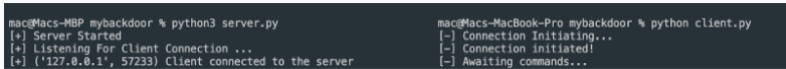
\includegraphics[height = 1 cm]{6.png}
\end{center}
Pentru a utiliza sqlmap, ar trebui să fii familiarizat cu diversele sale
Opțiuni. Cel mai simplu mod de a face acest lucru este să încerci să urmezi exemplele care
pot fi găsite pe Internet. Vă rugăm să citiți descrierea sqlmap după ce ați folosit software-ul deoarece acest lucru
va face posibilă înțelegerea documentului mai ușor. Apoi continuați cu hacking folosind sqlmap la următoarele
procese. Mai jos se vede cum are loc Procedeul de injectare SQL:\\
\begin{center}
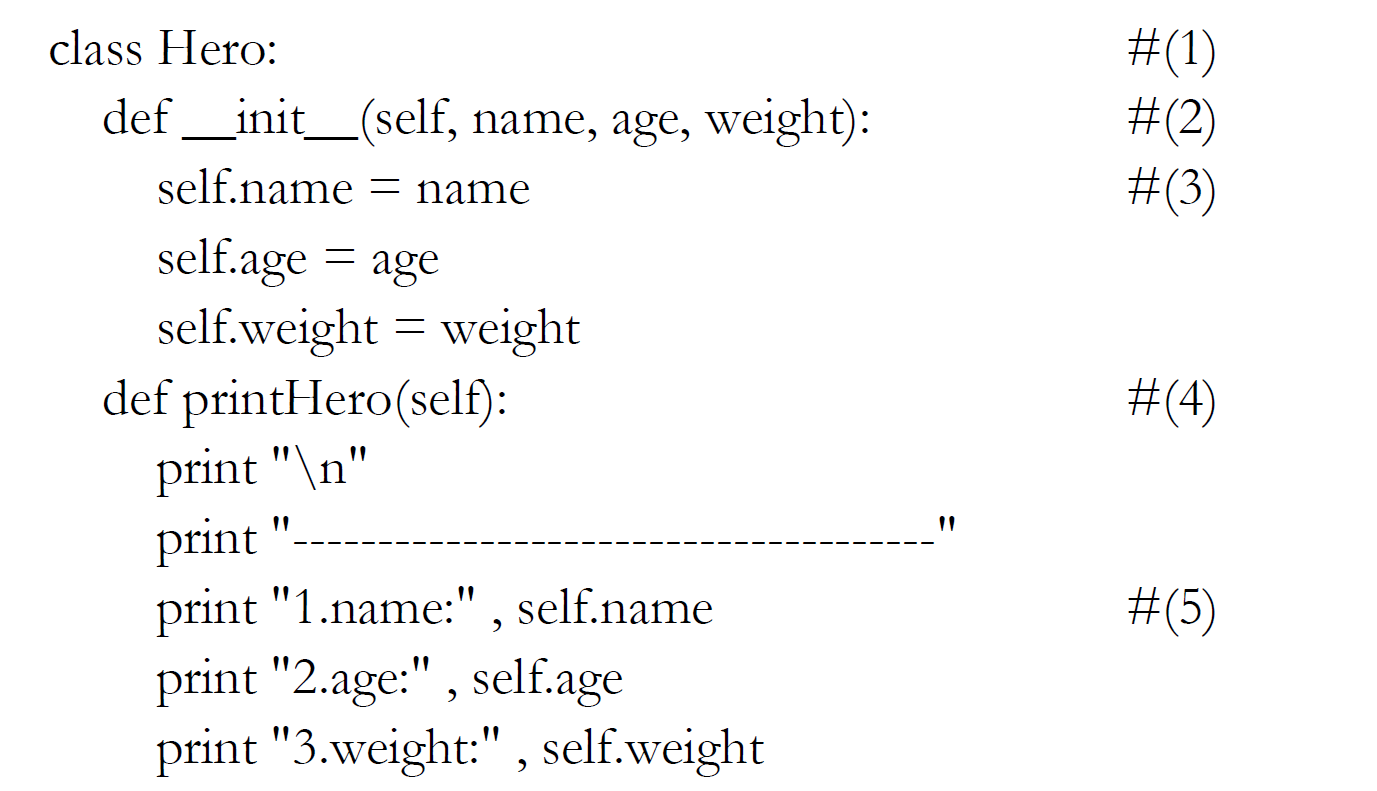
\includegraphics[height = 5 cm]{7.png}
\end{center}
Cu sqlmap, hacking-ul continuă pas cu pas. Site-ul Web este
analizat pentru a găsi vulnerabilități una câte una pornind de la simple
informații. Un atac SQL Injection este de obicei efectuat urmând cei cinci pași de mai jos.\\
\textbf{(1) Adresa URL de căutare:} un atac cu injecție SQL pirata sistemul
baza URL-ului. Atacă în principal funcția GET,
care trimite intrarea utilizatorului plasată după URL. Poți cu ușurință
căutați adresa URL țintă folosind Google. Pot fi diferite pagini
deschis pentru a observa modificarea adresei URL. În acest moment, unii
cunoștințele de HTML și JavaScript sunt utile.\\
\textbf{(2) Detectarea vulnerabilităților:} Programul ”sqlmap.py” poate fi
folosit pentru a detecta vulnerabilități în adresa URL. De la SQL Injection
Codul de protecție a fost aplicat la majoritatea programelor web,
vulnerabilitățile necesită colectarea multor URL-uri. URL-uri către
detectarea vulnerabilităților poate fi colectată folosind instrumente automate,
cum ar fi un crawler Web. Un crawler web primește codul sursă
pentru site-ul web și extrage adresele URL corespunzătoare.\\
\textbf{(3) Tabel de căutare:} dacă sunt detectate vulnerabilități în adresa URL,
hackerul poate căuta în tabelele din baza de date utilizând
sqlmap. Numele tabelului poate oferi importante informații.\\
\textbf{(4) Coloana de căutare}: În primul rând, selectați tabelul și căutați
coloană conținută în acesta. Numele coloanei este făcut să reflecte
caracteristicile datelor. Prin urmare, este posibil să se facă ușor
găsiți o coloană care conține informații importante.\\
\textbf{(5) Căutarea datelor}: Selectați o coloană pentru a interoga datele conținute
acolo. Dacă datele sunt criptate, sqlmap poate folosi dicționar
tehnici de atac pentru decriptarea datelor.
Puteți utiliza un crawler Web, așa că să presupunem că ați găsit un
URL vulnerabil. Adresa URL vulnerabilă este un ”config.php” care oferă
informațiile de mediu ale pluginului WordPress. Atunci sa
detectam vulnerabilități în acea adresă URL. Executați programul înCommand prompt și trecem la directorul ”C:\Python27\sqlmap”. Apoi introducem următoarea comandă
\begin{center}
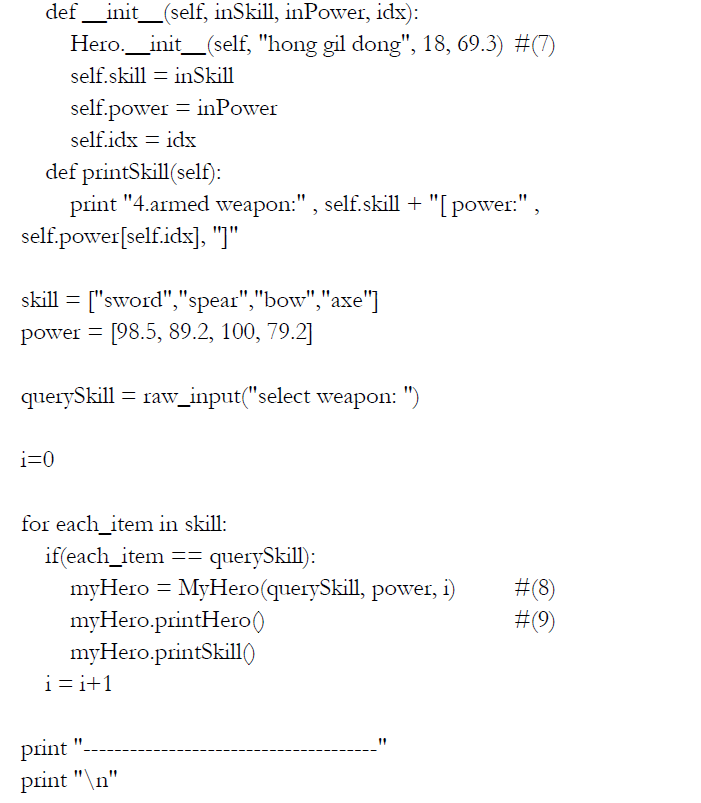
\includegraphics[height = 1 cm]{8.png}
\end{center}
\section{Password Cracking Attack}
Python este similar cu Java, PHP și ASP prin faptul că o pagină Web poate și
fi apelata când rulează un program. Punctele forte ale lui Python este că poate
crea un program simplu cu câteva linii de cod. Capacitatea de a accesa
pagina web din aplicație oferă capacitatea de automatizare
a diverselor operatii. Mai întâi, să învățăm procesul de a apela o pagină web
cu Python.
O aplicație Python poate apela o pagină web într-un mod simplu utilizând
modulele ”urllib” și ”urllib2”. ”urllib” creează mesaje POST
în același mod ca ”key1=value1&key2=value2”. În ”urllib2”,
puteți crea un obiect ”Solicitare”, care returnează un obiect ”Răspuns”.
printr-un apel către serverul Web. Procedura pas cu pas este următoarea.
(1) Obiect de solicitare: Folosind modulul ”urllib”, puteți crea un
Antet HTTP și date Corp. Când trimiteți comanda ”GET”, un obiect ”Solicitare” nu este creat separat. Doar
URL care este în caracter atunci când se apelează transportul HTTP.\\
(2) Transferul HTTP: Funcțiile furnizate de ”urllib2” pot
poate fi folosite pentru a apela imediat adresa URL, fără nimic suplimentar. URL-ul este transmis ca un
argument și obiectul ”Solicitare” este transmis împreună, dacă este necesar.
Această funcție acceptă majoritatea caracteristicilor furnizate de a
browser pentru a furniza comunicarea.\\
(3) Server PC: URL-ul indică un serviciu care rulează pe un Apache
Server web pe serverul PC. Serverul Web Apache analizează
Antetul și Corpul HTTP și apoi invocă cele dorite
serviciu. Rezultatele sunt apoi trimise înapoi la computerul hackerului de către
crearea unui format de protocol HTTP.\\
(4) Obiectul răspunsului: Răspunsul de la serverul web este un
Format de protocol HTTP. Modulul ”urllib2” returnează
Obiectul ”Răspuns” care poate fi utilizat în această aplicație.\\
(5) Hacker PC: puteți interoga adresa URL de returnare, codul de stare HTTP,
și informațiile și datele antetului utilizând funcțiile acelui obiect „Răspuns” pe care le oferă.\\
Hackingul necesită sarcini repetitive, deci dacă utilizați un browser
pentru a sparge direct un site Web, este necesar să faceți clic în mod repetat în timp ce faceti
modificarea continuă a valorilor de intrare. Cu toate acestea, dacă este posibil
implementați acest proces într-un program si veti putea reuși doar cu a
câteva linii de cod. Prin urmare, să învățăm cum Python apelează o pagină Web
prin exemplul următor.
\begin{center}
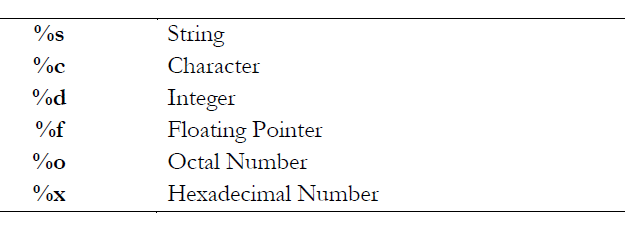
\includegraphics[height = 5 cm]{9.png}
\end{center}
Compilati pana la functionare exemplul de mai sus.
\section{Bibliografie}
Python Hacking Essentials Paperback 2015 by Earnest Wish, \\
https://www.amazon.com/Python-Hacking-Essentials-Earnest-Wish/dp/1511797568\\
https://www.geeksforgeeks.org/socket-programming-python/


\end{document}
